\documentclass{article}
\usepackage[utf8]{inputenc} % allow utf-8 input
\usepackage[T1]{fontenc}    % use 8-bit T1 fonts
\usepackage{hyperref}       % hyperlinks
\usepackage{url}            % simple URL typesetting
\usepackage{booktabs}       % professional-quality tables
\usepackage{amsfonts}       % blackboard math symbols
\usepackage{nicefrac}       % compact symbols for 1/2, etc.
\usepackage{microtype}      % microtypography

\usepackage[english]{babel}
\usepackage{blindtext}
\usepackage{bm}
\usepackage{index}
\usepackage[utf8]{inputenc}
\usepackage{graphicx}
\graphicspath{ {./} }
\usepackage{amsmath}
\usepackage{amssymb}
\usepackage{listings}
\usepackage{color}
\usepackage{siunitx}
\usepackage{longtable}

\definecolor{dkgreen}{rgb}{0,0.6,0}
\definecolor{gray}{rgb}{0.5,0.5,0.5}
\definecolor{mauve}{rgb}{0.58,0,0.82}

\lstset{frame=tb,
  language=Python,
  aboveskip=3mm,
  belowskip=3mm,
  showstringspaces=false,
  columns=flexible,
  basicstyle={\small\ttfamily},
  numbers=none,
  numberstyle=\tiny\color{gray},
  keywordstyle=\color{blue},
  commentstyle=\color{dkgreen},
  stringstyle=\color{mauve},
  breaklines=true,
  breakatwhitespace=true,
  tabsize=3
}
%% ========New command added by Han Liu===========================
\renewcommand{\vec}[1]{\boldsymbol{#1}}
\newenvironment{qparts}{\begin{enumerate}[1.]}{\end{enumerate}}
\usepackage{amsmath,textcomp,amssymb,geometry,graphicx,enumerate}
\usepackage{subcaption}
\usepackage[figurename=Fig.,labelfont=bf,labelsep=period]{caption}
\usepackage[capitalise]{cleveref}
\usepackage[ruled,vlined]{algorithm2e}
%% ===============================================================

\begin{document}
\title{EECS289A Introduction to Machine Learning,  Project T Final - Quiz Questions}
\author{%
  \ Han Liu, \ Peng Tan, \ Dilu Xu, \ Jinyan Zhao \\
  Department of Civil Engineering\\
  Universitu of California, Berkeley\\
  Berkeley, CA 94704 \\
  \texttt{\{han\_liu, tanpeng, diluxu, jinyan\_zhao\}@berkeley.edu} \\
}
\maketitle

\section{Basic Question}
\begin{qparts}
\item  A computer program is said to learn from experience E with respect to some task T and some performance measure P if its performance on T, as measured by P, improves with experience E.\\
 Suppose we feed a learning algorithm a lot of historical weather data, and have it learn to predict weather. What would be a reasonable choice for P? \\
a. The probability of it correctly predicting a future date’s weather.\\
b. The weather prediction task.\\
c. The process of the algorithm examining a large amount of historical weather data.\\
d. None of these.\\
\underline{\textbf{Answer:}}\\
a


 \item  A computer program is said to learn from experience E with respect to some task T and some performance measure P if its performance on T, as measured by P, improves with experience E. \\
 Suppose we feed a learning algorithm a lot of historical weather data, and have it learn to predict weather. In this setting, what is T?\\
 a. The weather prediction task.\\
b. The probability of it correctly predicting a future date’s weather.\\
c. The process of the algorithm examining a large amount of historical weather data.\\
d. None of these.\\
 
\underline{\textbf{Answer:}}\\
a

 \item  Suppose you are working on weather prediction, and use a learning algorithm to predict tomorrow’s temperature (in degrees Centigrade/Fahrenheit).\\
Would you treat this as a classification or a regression problem?\\
a. Regression\\
b. Classification\\
 
\underline{\textbf{Answer:}}\\
a

 \item  Suppose you are working on weather prediction, and your weather station makes one of three predictions for each day’s weather: Sunny, Cloudy or Rainy. You’d like to use a learning algorithm to predict tomorrow’s weather.\\
Would you treat this as a classification or a regression problem?\\
a. Regression\\
b. Classification\\
 
\underline{\textbf{Answer:}}\\
b

\end{qparts}


\newpage
\section{Elastic Net}
In class we discussed two types of regularization, $l_1$ and $l_2$. Both are useful, and sometimes it is helpful combine them, giving the objective function below (\textbf{in this problem we have excluded} $w_0$ \textbf{for simplicity}):
\begin{equation}
F(\vec{w}) = \frac{1}{2}\sum^n_{j=1}(y^{(j)}-\sum^d_{i=1}\vec{w}_i\vec{x}_i^{(j)})^2+\alpha\sum^d_{i=1}|\vec{w}_i|+\frac{\lambda}{2}+\sum^d_{i=1}\vec{w}_i^2
\end{equation}
Here, $(\vec{x}^{(j)},y^{(j)})$ is j-th example in the training data, w is a d dimensional weight vector, $\lambda$ is a regularization parameter for the $l_2$ norm of w, and $\alpha$ is a regularization parameter for the $l_1$ norm of w. This approach is called the Elastic Net, and you can see that it is a generalization of Ridge and Lasso regression: It reverts to Lasso when $\lambda = 0$, and it reverts to Ridge when $\alpha = 0$. In this question, we are going to derive the coordinate descent (CD) update rule for this objective.

Let g, h, c be real constants, and consider the function of x
\begin{equation}
f_1(x) = c+gx+\frac{1}{2}hx^2
\end{equation}
\begin{qparts}
\item {[}4 points{]} 
What is the $x^*$ that minimizes $f_1(x)$? (i.e. calculate $x^*=\arg\min f_1(x)$)\\
\underline{\textbf{Answer:}}\\
Take the gradient of $f_1(x)$ and set it to 0.
\begin{alignat}{2}
g+hx&=0 \\
x^*&=-\frac{g}{h}
\end{alignat}   

Let $\alpha$ be an additional real constant, and consider another function of x
\begin{equation}\label{eq:hl1}
f_2(x) = c+gx+\frac{1}{2}hx^2+\alpha|x|(h>0, \alpha>0)
\end{equation}
This is a piecewise function, composed of two quadratic functions:
\begin{equation}
f_2^-(x) = c+gx+\frac{1}{2}hx^2-\alpha x
\end{equation}
and
\begin{equation}
f_2^+(x) = c+gx+\frac{1}{2}hx^2+\alpha x
\end{equation}
Let $\tilde{x}^-=\arg\min_{x\in\mathbb{R}}f_2^-(x)$ and $\tilde{x}^+=\arg\min_{x\in\mathbb{R}}f_2^+(x)$.\\
(\textbf{Note:} The argmin is taken over $(-\infty, +\infty)$ here.
\\

\item {[}6 points{]} 
What are $\tilde{x}^+$ and $\tilde{x}^+$? Show that $\tilde{x}^-\geq\tilde{x}^+$. \\
\underline{\textbf{Answer:}}\\
Using the answer from part 1), we get $\tilde{x}^+=-\frac{g+\alpha}{h}$ and $\tilde{x}^-=-\frac{g-\alpha}{h}$. Since $\tilde{x}^--\tilde{x}^+=\frac{2\alpha}{h}\geq 0$, we have $\tilde{x}^-\geq\tilde{x}^+$.


\item {[}12 points{]} 
Draw a picture of $f_2(x)$ in each of the three cases below:
\begin{enumerate}[(a)]
\item $\tilde{x}^->0$, $\tilde{x}^+>0$
\item $\tilde{x}^-<0$, $\tilde{x}^+<0$
\item $\tilde{x}^->0$, $\tilde{x}^+<0$
\end{enumerate}
For each case, mark the minimum as either 0, $\tilde{x}^-$, or $\tilde{x}^+$. (You do not need to draw perfect curves, just get the rough shape and the relative locations of the minima to the x-axis)\\
\underline{\textbf{Answer:}}\\
\cref{fig:hl1} gives the example picture of three cases. To understand the answer, note the following:
\begin{itemize}
\item $f^+_2(0)=f^-_2(0)$, this means the two piece of $f_2$ match each other at x = 0.
\item When $\tilde{x}^-\geq 0$, the minimum of the left part is at 0, i.e. $\arg\min_{x\in \left(-\infty, 0\right]}f_2^-(x)=0$
\item When $\tilde{x}^-\leq 0$, the minimum of the left part is at $\tilde{x}^-$, i.e. $\arg\min_{x\in \left(-\infty, 0\right]}f_2^-(x)=\tilde{x}^-$
\item Similar rules holds for the right part of the curve.
\end{itemize}
\begin{figure*}[!htb]
    \centering
    \begin{subfigure}[t]{0.31\textwidth}
        \centering
        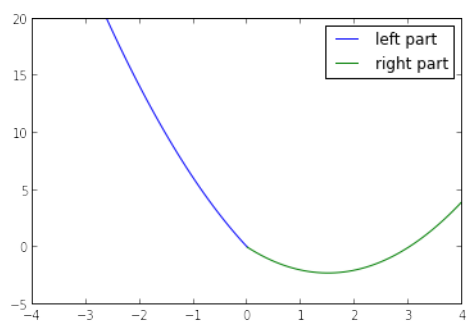
\includegraphics[height=1.3in]{fig/fig-han-1.PNG}
        \caption{$\tilde{x}^->0$, $\tilde{x}^+>0$, the minima is at $\tilde{x}^+$.}
    \end{subfigure}%
    ~
    \begin{subfigure}[t]{0.31\textwidth}
        \centering
        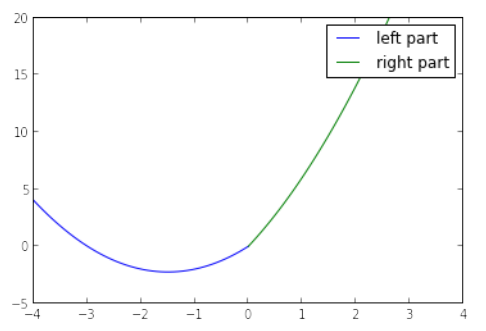
\includegraphics[height=1.3in]{fig/fig-han-2.PNG}
        \caption{$\tilde{x}^-<0$, $\tilde{x}^+<0$, the minima is at $\tilde{x}^-$.}
    \end{subfigure}
    ~
    \begin{subfigure}[t]{0.31\textwidth}
        \centering
        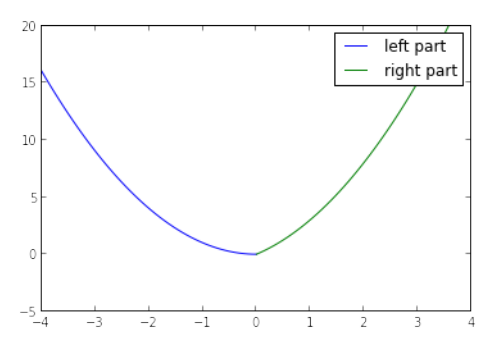
\includegraphics[height=1.3in]{fig/fig-han-3.PNG}
        \caption{$\tilde{x}^->0$, $\tilde{x}^+<0$, the minima is at 0.}
    \end{subfigure}
    \caption{Example picture of three cases.}
    \label{fig:hl1} 
\end{figure*}
\end{qparts}


\newpage
\section{Elastic Net Plus}
\begin{qparts}
\item {[}8 points{]} 
Write $x^*$, the minimum of $f_2(x)$, as a piecewise function of g. (Hint: what is
g in the cases above?)\\
\underline{\textbf{Answer:}}\\
Summarizing the result from the previous question, we have
\begin{equation}
x^*=
\begin{cases}
\tilde{x}^+ &\text{if $\tilde{x}^+>0$}\\
\tilde{x}^- &\text{if $\tilde{x}^-<0$}\\
0 &\text{if $\tilde{x}^+<0, \tilde{x}^->0$}
\end{cases}
\end{equation}
This is equivalent to the soft-threshold function
\begin{equation}
x^*=
\begin{cases}
   -\frac{g+\alpha}{h} &\text{if $g<-\alpha$}\\
   0 &\text{if $g\in\left[-\alpha, \alpha\right]$}\\
   -\frac{g-\alpha}{h} &\text{if $g>\alpha$}
   \end{cases}
\end{equation}

\item {[}8 points{]} 
Now let’s derive the update rule for $w_k$. Fixing all parameters but $w_k$, express the objective function in the form of Eq.~\eqref{eq:hl1} (here $w_k$ is our x). You do not
need to explicity write constant factors, you can put them all together as c. What are
g and h? Then putting it all together, write down the coordinate descent algorithm for the Elastic Net (\textbf{again excluding} $w_0$). You can write the update for $w_k$ in terms of the g and h you calculated in the previous question.\\
\underline{\textbf{Answer:}}\\
\begin{equation}
g=\sum^n_{j=1}x^{(j)}_k(\sum_{i\neq k}\vec{w}_i\vec{x}_i^{(j)}-y_i)
\end{equation}
\begin{equation}
h=\lambda+\sum^n_{j=1}(x^{(j)})^2
\end{equation}
The algorithm is shown in Algorithm.~\ref{algo:hl1}. You can compare it to the CD algorithm for Lasso, the only difference is adding $\lambda$ to h.\\
\begin{algorithm}[H]\label{algo:hl1}
\SetAlgoLined
% \KwResult{Write here the result }
%  initialization\;
 \While{not converged}{
  % instructions\;
  \For{$k\in \{1,2,\cdots,d\}$}{
   $g=\sum^n_{j=1}x^{(j)}_k(\sum_{i\neq k}\vec{w}_i\vec{x}_i^{(j)}-y_i)$\;
   $h=\lambda+\sum^n_{j=1}(x^{(j)})^2$\;
   $w_k=\begin{cases}
   -\frac{g+\alpha}{h} &\text{if $g<-\alpha$}\\
   0 &\text{if $g\in\left[-\alpha, \alpha\right]$}\\
   -\frac{g-\alpha}{h} &\text{if $g>\alpha$}
   \end{cases}$\;
   }{
   % instructions3\;
  }
 }
 \caption{Coordinate Descent for Elastic Net}
\end{algorithm}
\end{qparts}

\newpage
\section{True or False questions}
Answer True or False. Justify your answer very briefly in 1-2 sentences.
\begin{qparts}
\item Increasing the regularization parameter $\lambda$ in lasso regression leads to sparser regression coefficients.
\underline{\textbf{Answer:}}\\
True. Larger regularization parameter penalizes non-zero coefficients more, leading to
sparser solution.

\item In Lasso regression, can the regulariser increase the sparsity of the resulting solutions?\\
\underline{\textbf{Answer:}}\\
True, Lasso introduces the L1 norm penalty, so increasing the penalty will cause more and more of the parameters to be driven to zero. As seen in \cref{fig:hl2}, where the red contours are representing the error function and the solid blue areas the constraint regions for the parameters, in the Lasso case, the function is likely to hit the constraint region on one of the four corners. This will make a parameter equal with zero.
\begin{figure}[!htb]
    \centering
    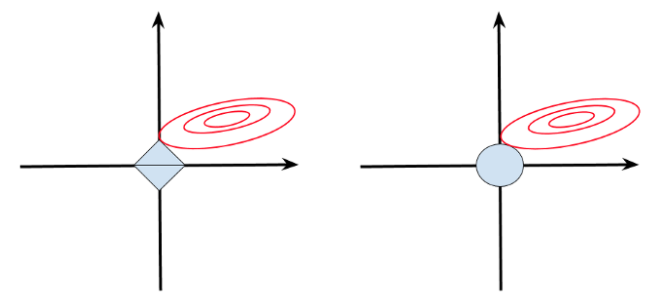
\includegraphics[width=.6\textwidth]{fig/fig-han-4.PNG}
    \caption{Spam-Estimation picture for the LASSO (left) and Ridge regression (right).}
    \label{fig:hl2}
\end{figure}

\item Is the objective of Lasso regression differentiable and convex?\\
\underline{\textbf{Answer:}}\\
False, it is not differentiable. As Lasso uses L1 norm penalty, this L1 loss function is defined based on the absolute value of the difference between two values. Since the loss function is a modulus function, there will exist an inflection point where the slope cannot be computed and the function is not differentiable. In contrast, for the case of Ridge regression, where we use L2 norm penalty, we can get the slope at any point and the objective is differentiable.

\item Are the objectives of Ridge and Lasso regression both convex and have closed-form solutions?\\
\underline{\textbf{Answer:}}\\
False, they are both convex, but Lasso does not always have a closed-form solution. LASSO regression must be solved numerically by using quadratic programming or more general convex optimisation methods.

\item Is it true that the L1 term in Lasso has the following purposes: performing feature selection, compensating for overfitting and smoothing?\\
\underline{\textbf{Answer:}}\\
False. The first two purposes are true, but not the last one. As it is mentioned early, both L1 and L2 terms are introduced to compensate for overfitting. By making the parameters equal with zero, the L1 norm discards some features and, thus, performs feature selection. In terms of smoothing, we cannot say L1 has this purpose, as the L1 loss function does not have continuous derivatives.
\end{qparts}


\newpage
\section{Quick questions}
Explain \textbf{in one or two sentences} why the statements are true (or false).
\begin{qparts}
\item L2 loss is more robust to outliers than L1 loss.\\
\underline{\textbf{Answer:}}\\
False \\
The gradient of L2 loss can grow without bound whereas the L1 loss gradient is bounded, hence the influence of an outlier is limited.

\item Logistic loss is better than L2 loss in classification tasks.\\
\underline{\textbf{Answer:}}\\
True \\ 
With logistic loss, correctly classified points that are far away from the decision boundary have much less impact on the decision boundary.


\item In terms of feature selection, L2 regularization is preferred since it comes up with sparse solutions.\\
\underline{\textbf{Answer:}}\\
False \\
L1 regularization (LASSO) comes up with sparse solutions due to nonvanishing gradient at 0.
\end{qparts}


\newpage
\section{Gradient descent}
Denote by $\vec{x}\in\mathbb{R}^d$ data, by $\vec{w}\in\mathbb{R}^d$ the weight vector, by $y\in\mathbb{R}y$ lables, by $\lambda>0$ a regularization constant, and by m the total number of data points. Let R(w) be the regularized risk function:
\begin{equation}
R(w):=\frac{1}{m}\sum^m_{i=1}l(y_i-\left<w,x_i\right>)+\frac{\lambda}{2}||\vec{w}||^2 \quad\text{where}\quad l(\xi)=\begin{cases}
\frac{1}{2}\xi^2 &\text{if $|\xi|<1$} \\
|\xi|-\frac{1}{2} &\text{otherwise}
\end{cases}
\end{equation}
\begin{qparts}
\item Calculate the batch gradient of R(w) with respect to w.\\
\underline{\textbf{Answer:}}\\
Define $g_i$ as the gradient of ith data point.
\begin{equation}
g_i=\begin{cases}
(\left<w,x_i\right>-y)x_i &\text{if$|\left<w,x_i\right>-y|<1$} \\
\text{sgn}(\left<w,x_i\right>-y)x_i &\text{otherwise}
\end{cases}
\end{equation}
\begin{equation}
\frac{\partial R}{\partial w}=\frac{1}{m}\sum^m_{i=1}g_i+\lambda w
\end{equation}

\item Write out a stochastic gradient descent learning algorithm for minimizing R(w).\\
\underline{\textbf{Answer:}}\\
Randomly select a training instance $x_i$, update w as follows:
\begin{equation}
\vec{w}\leftarrow (1-\lambda\eta_t)\vec{w}-\eta_tg_i
\end{equation}

\item Name two common choices for choosing the learning rate and briefly explain their properties.\\
\underline{\textbf{Answer:}}\\
$O(\frac{1}{\sqrt{t}}), O(\frac{1}{t})$ for strong convexity, Polynomial decay, AdaGrad, etc.
\end{qparts}

\newpage
\section{Logistic Regression}

\begin{qparts}
 \item For logistic regression, the gradient is given by $\frac{\partial }{\partial \theta_j } J(\theta) = \frac{1}{m} \sum_{i=1}^{m}(h_\theta(x^{(i)})-y^{i})x^{(i)}_j$. Which of these is a correct gradient descent update for logistic regression with a learning rate of $\alpha$? \\
 Check all that apply.\\
 a. $\theta_j := \theta_j - \alpha \frac{1}{m} \sum_{i=1}^m (h_\theta(x^{(i)-y^i}) x^{(i)}_j$ (simultaneously update for all j).\\
 b. $\theta := \theta - \alpha \frac{1}{m} \sum_{i=1}^m (\theta^Tx-y^{(i)}) x^{(i)}$.\\
 c. $\theta_j := \theta_j - \alpha \frac{1}{m} \sum_{i=1}^m \left(\frac{1}{1+e^{-\theta^Tx^{(i)}}}-y^{(i)}\right) x^{(i)}_j$ (simultaneously update for all j).\\
 d. $\theta_j := \theta_j - \alpha \frac{1}{m} \sum_{i=1}^m (h_\theta(x^{(i)-y^i}) x^{(i)}$ (simultaneously update for all j).\\
 
\underline{\textbf{Answer:}}\\
ac

 \item Suppose that you have trained a logistic regression classifier, and it outputs on a new example a prediction $h_\theta(x) = 0.2$. This means (check all that apply):\\
a. Our estimate for $P(y = 1|x; \theta)$ is 0.8.\\
b. Our estimate for $P(y = 0|x; \theta)$ is 0.8.\\
c. Our estimate for $P(y = 1|x; \theta)$ is 0.2.\\
d. Our estimate for $P(y = 0|x; \theta)$ is 0.2.\\
 
\underline{\textbf{Answer:}}\\
bc

\end{qparts}

\newpage
\section{Multiple choice I}
In this part, you only need to choose one correct answer.
\begin{qparts}
\item You run gradient descent for 15 iterations with $\alpha = 0.3$ and compute after each iteration. You find that the value of $J(\theta)$ decreases slowly and is still decreasing after 15 iterations. Based on this, which of the following conclusions seems most plausible?\\
 a. Rather than use the current value of  $\alpha$, it’d be more promising to try a larger value of $\alpha$ (say $\alpha = 1.0$).\\
 b. Rather than use the current value of $\alpha$, it’d be more promising to try a smaller value of $\alpha$ (say $\alpha = 0.1$).\\
 c. $\alpha = 0.3$ is an effective choice of learning rate.\\
\underline{\textbf{Answer:}}\\
a
\item You run gradient descent for 15 iterations with $\alpha = 0.3$ and compute after each iteration. You find that the value of $J(\theta)$ decreases quickly then levels off. Based on this, which of the following conclusions seems most plausible?\\
 a. Rather than use the current value of  $\alpha$, it’d be more promising to try a larger value of $\alpha$ (say $\alpha = 1.0$).\\
 b. Rather than use the current value of $\alpha$, it’d be more promising to try a smaller value of $\alpha$ (say $\alpha = 0.1$).\\
 c. $\alpha = 0.3$ is an effective choice of learning rate.\\
\underline{\textbf{Answer:}}\\
c

\item Suppose you have $m = 23$ training examples with $n = 5$ features (excluding the additional all-ones feature for the intercept term, which you should add). The normal equation is $\theta = (X^{T} X)^{-1}X^{T}y$. For the given values of m and n, what are the dimensions of $\theta$, X, and y in this equation?\\
a. X is 23 × 5, y is 23 × 1, $\theta$ is 5 × 5\\
b. X is 23 × 6, y is 23 × 6, $\theta$ is 6 × 6\\
c. X is 23 × 6, y is 23 × 1, $\theta$ is 6 × 1\\
d. X is 23 × 5, y is 23 × 1, $\theta$ is 5 × 1\\
\underline{\textbf{Answer:}}\\
c\\
 X has m rows and n+1 columns (+1 because of the $x_0=1$ term). y is m-vector. $\theta$ is an $(n+1)$-vector


\item Suppose you have a dataset with $m = 1000000$ examples and $n = 200000$ features for each example. You want to use multivariate linear regression to fit the parameters $\theta$ to our data. Should you prefer gradient descent or the normal equation?\\
a. Gradient descent, since it will always converge to the optimal $\theta$.\\
b. Gradient descent, since $(X^T X)^{-1} $will be very slow to compute in the normal equation.\\
c. The normal equation, since it provides an efficient way to directly find the solution.\\
d. The normal equation, since gradient descent might be unable to find the optimal $\theta$.\\
\underline{\textbf{Answer:}}\\
b\\
With $n = 200000$ features, you will have to invert a $200001 x 200001$ matrix to compute the normal equation. Inverting such a large matrix is computationally expensive, so gradient descent is a good choice.
 
 \item Which of the following are reasons for using feature scaling?\\
a. It is necessary to prevent gradient descent from getting stuck in local optima.\\
b. It speeds up solving for $\theta$ using the normal equation.\\
c. It prevents the matrix $X^T X$ (used in the normal equation) from being non-invertable (singular/degenerate).\\
d. It speeds up gradient descent by making it require fewer iterations to get to a good solution.\\
\underline{\textbf{Answer:}}\\
d\\
For a, the cost function $J(\theta)$ for linear regression has no local optima. For b, the magnitute of the feature values are significant in terms of computational cost. For c, feature scaling has nothing to do with matrix inversion. For d, feature scaling speeds up gradient descent by avoiding many extra iterations that are required when one or more features takes on much larger values than he rest.
 
\end{qparts}


\newpage
\section{Multiple choice II}
In this part, some questions may have multiple correct answers.
\begin{qparts}

 \item Some of the problems below are best addressed using a supervised learning algorithm, and the others with an unsupervised learning algorithm. Which of the following would you apply supervised learning to? (Select all that apply.) In each case, assume some appropriate dataset is available for your algorithm to learn from.\\
 a. Given historical data of children’s ages and heights, predict children’s height as a function of their age.\\
 b. Given 50 articles written by male authors, and 50 articles written by female authors, learn to predict the gender of a new manuscript’s author (when the identity of this author is unknown).\\
 c. Take a collection of 1000 essays written on the US Economy, and find a way to automatically group these essays into a small number of groups of essays that are somehow “similar” or “related”.\\
 d. Examine a large collection of emails that are known to be spam email, to discover if there are sub-types of spam mail.\\
 
\underline{\textbf{Answer:}}\\
ab

 \item Some of the problems below are best addressed using a supervised learning algorithm, and the others with an unsupervised learning algorithm. Which of the following would you apply supervised learning to? (Select all that apply.) In each case, assume some appropriate dataset is available for your algorithm to learn from.\\
a. Given data on how 1000 medical patients respond to an experimental drug (such as effectiveness of the treatment, side effects, etc.), discover whether there are different categories or “types” of patients in terms of how they respond to the drug, and if so what these categories are.\\
b. Given a large dataset of medical records from patients suffering from heart disease, try to learn whether there might be different clusters of such patients for which we might tailor separate treatments.\\
c. Have a computer examine an audio clip of a piece of music, and classify whether or not there are vocals (i.e., a human voice singing) in that audio clip, or if it is a clip of only musical instruments (and no vocals).\\
d. Given genetic (DNA) data from a person, predict the odds of him/her developing diabetes over the next 10 years.\\
 
 \underline{\textbf{Answer:}}\\
cd


 \item Some of the problems below are best addressed using a supervised learning algorithm, and the others with an unsupervised learning algorithm. Which of the following would you apply supervised learning to? (Select all that apply.) In each case, assume some appropriate dataset is available for your algorithm to learn from.\\
a. Take a collection of 1000 essays written on the US Economy, and find a way to automatically group these essays into a small number of groups of essays that are somehow “similar” or “related”.\\
b. Given genetic (DNA) data from a person, predict the odds of him/her developing diabetes over the next 10 years.\\
c. Examine a large collection of emails that are known to be spam email, to discover if there are sub-types of spam mail.\\
d. Examine the statistics of two football teams, and predict which team will win tomorrow’s match (given historical data of teams’ wins/losses to learn from).\\
 
 \underline{\textbf{Answer:}}\\
bc


 \item Which of these is a reasonable definition of machine learning?\\
a. Machine learning is the science of programming computers.\\
b. Machine learning learns from labeled data.\\
c. Machine learning is the field of allowing robots to act intelligently.\\
d. Machine learning is the field of study that gives computers the ability to learn without being explicitly programmed.\\
 
 \underline{\textbf{Answer:}}\\
d

\end{qparts}

\newpage
\section{Extra Question}
\begin{qparts}

 \item Which of the following statements about regularization are true? Check all that apply.\\
a. Using a very large value of $\lambda$ hurt the performance of your hypothesis; the only reason we do not set $\lambda$ to be too large is to avoid numerical problems.\\
b. Because logistic regression outputs values$ 0 \leq h_\theta(x) \leq 1$, its range of output values can only be “shrunk” slightly by regularization anyway, so regularization is generally not helpful for it.\\
c. Consider a classification problem. Adding regularization may cause your classifier to incorrectly classify some training examples (which it had correctly classified when not using regularization, i.e. when $\lambda$ = 0).\\
d. Using too large a value of $\lambda$ can cause your hypothesis to overfit the data; this can be avoided by reducing $\lambda$.\\
 \underline{\textbf{Answer:}}\\
 c

 \item Which of the following statements about regularization are true? Check all that apply.\\
a. Using a very large value of $\lambda$ hurt the performance of your hypothesis; the only reason we do not set $\lambda$ to be too large is to avoid numerical problems.\\
b. Because logistic regression outputs values$ 0 \leq h_\theta(x) \leq 1$, its range of output values can only be “shrunk” slightly by regularization anyway, so regularization is generally not helpful for it.\\
c. Because regularization causes $J(\theta)$ to no longer be convex, gradient descent may\\
d. Using too large a value of $\lambda$ can cause your hypothesis to underfit the data; this can be avoided by reducing $\lambda$.\\
 \underline{\textbf{Answer:}}\\
d


\end{qparts}
\end{document}